\documentclass[sigconf]{acmart}

\usepackage[english]{babel}
 \usepackage{booktabs}
 \usepackage{graphicx}
 \usepackage{subcaption}
 \usepackage{url}
\usepackage{blindtext}
\usepackage{dirtytalk}
\usepackage[linesnumbered]{algorithm2e}
\newcommand{\etal}{\textit{et al.} }
\newcommand{\smartnic}{\textit{SmartNIC} }
\newcommand{\smartnics}{\textit{SmartNICs} }
\begin{document}
\title{In depth in-network neural network performance analysis}

%\titlenote{Produces the permission block, and copyright information}
%\subtitle{Extended Abstract}
   
%   \streetaddress{Address}
%   \city{City} 
%   \state{State} 
%   \postcode{Zipcode}
% }
% \email{email@domain.com}
\author{Hesam Tajbakhsh}
% \authornote{Note}
\orcid{0002-8100-4323}
\affiliation{%
  \institution{Dalhousie University}
%   \streetaddress{Address}
  \city{Halifax} 
  \state{Nova Scotia} 
%   \postcode{Zipcode}
}
\email{hs762129@dal.ca}


\begin{abstract}
\textcolor{red}{[add abstract]}

In this project, we investigate running neural networks on \smartnics without any accuracy loss. Previous works modified their neural networks to be compatible with their \smartnics due to their device's limitation. Our goal is to figure out if we can execute an accurate model on a different \smartnic to release some tasks from the host and gain the same or even better performance.
\end{abstract}

\maketitle

\section{Introduction}
Reconfigurable network cards- or in other words \smartnics, offering more resources in datacenters, are becoming increasingly popular in recent years. There are several kinds of \smartnic, and in this report, first, we will briefly introduce two main architectures of them and their advantages. Afterward, we will review Artificial Neural Networks (ANN) to provide adequate background for our work. This work will focus on executing Machine Learning (ML) and Deep Learning (ML) applications on \smartnics. Our primary reference \cite{siracusano2020running} has examined ML/DL Neural Networks (NNs) on two types of \smartnics, but they penalized some parameters (e.g., the accuracy of NNs); however, the throughput and latency are enhanced significantly.
\par
By and large, each \smartnic has its limitations and advantages. We aim to figure out whether we can execute these applications on a \smartnic without sacrificing the accuracy. So, we will pick the \smartnic which has not been investigated for these purposes and investigate if the \smartnic helps us to achieve our goal or not. Our results show the selecting the suitable model for our \smartnic's type is crucial due to its limitation. We will evaluate two types of ANNs, and yield some information showing which one can be a better fit than the other.

\par
With this in mind, the rest of the article is organized as the following. In section \ref{sec-back}, \smartnics are introduced. We will also talk about artificial neural networks in section \ref{sec-back}. In \ref{sec-motive} we talk about offloading ANN into \smartnics and explain our goal. Our testbed details and results are studied in sections \ref{sec-testbed} and \ref{sec-results}, respectively. Then, we will address a few related works in section \ref{sec-related}. Eventually, in section \ref{sec-conlcu}, we will conclude our project based on the provided results.

\section{Background}
\label{sec-back}
We divide this section into two parts; introducing \smartnics briefly and improving the overall performance by \smartnics are discussed in the first part.  Then, we talk about Artificial Neural Networks (ANN) in the second part.

\subsection{\smartnics Overview}
A glance at Fig. \ref{arhs} reveals two architectures for \smartnics. In the first architecture, \smartnic's processing is located on the path of networking, while in the latter one, Fig. \ref{off-path}, the processing unit is located off the path, communicating with the NIC and the host through PCI Express slot (Peripheral Component Interconnect Express). There are several choices for the \smartnic's processing unit. On-the-shelve CPUs, FPGA, and ASIC are some instances that can be mounted on the \smartnics. In the case of general-purpose CPUs, most of them are ARM-based or MIPS-based wimpy processors.

\par
Owing to the high bandwidth demands of \smartnics, they are connected to hosts over the PCI Express slot, as mentioned in the previous paragraph. However,  PCI Express prompts for extra latency overhead in some cases. Keeping this in mind, either executing an application or offloading part of it into on-path \smartnics can exclude PCI Express extra latency. Nevertheless, FPGAs and CPUs used in on-path \smartnics have limited resources and capabilities. For example, they usually do not support floating-point operations or have a limited memory footprint. It goes without saying that offloaded applications should be modified to be compatible with \smartnics environments and may lose some traits. We will talk about different techniques of modification in the second half of this section, where we discuss ANNs.
\par
Worth to mention, for each kind of \smartnics there are a few brands available in the market; some of them are listed in Table \ref{brands}.

\begin{figure}[ht!]
\centering
    \begin{subfigure}{0.23\textwidth}
        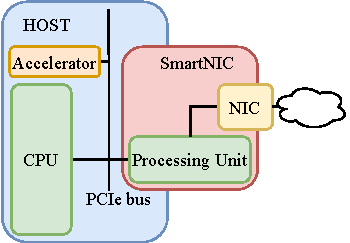
\includegraphics[width=\textwidth]{./figs/on-path.pdf}
        \caption{On-path Architecture}
        \label{on-path}
    \end{subfigure}\hfil
    \begin{subfigure}{0.23\textwidth}
        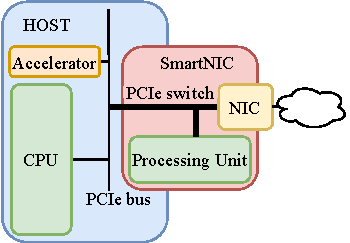
\includegraphics[width=\textwidth]{./figs/off-path.pdf}
        \caption{Off-path Architecture}
        \label{off-path}
    \end{subfigure}\hfil
    \caption{Two architectures for \smartnics}
\label{arhs}
\end{figure}

\begin{table}[hbt!]
\caption{A Few \textit{SmartNICs} Available in the Market}
\label{brands}
\begin{tabular}{|c|c|}
\hline
                   & Available Brands in the Market \\ \hline
On-Path FPGA-based & NetFGPA-SUME \cite{netfpga-sume}                  \\ \hline
On-Path CPU-based  & Liquid IO \cite{liquidio}                     \\ \hline
Off-Path CPU-based & Stingray \cite{stingray} and BlueField \cite{bluefield}        \\ \hline
\end{tabular}
\end{table}

%\subsection{DNNs}
\subsection{Artificial Neural Networks (ANNs)}
\textcolor{red}{[Let's focus our analyses on deep neural networks (DNNs) as these are currently more appealing. Give some background on them. What is a DNN? Where are they used (i.e., most common applications)? What about networking use cases? Give an overview about different architectures (i.e., show they are pretty varied - CNN, RNN, GNN, fully  NN). Talk about different flavors (prunned, compressed, quantized)]}
\textcolor{blue}{Personally, I prefer ANN rather than DNN since some of our implementations are ANN, not necessarily DNN}

In a nutshell, an artificial neural network- or ANN as we call in the rest of the report-is a network of neurons connecting with weighted vertices. An ANN can have one or more than one hidden layer. Also, the nodes/layers can organize different topologies. For instance, Fig. \ref{fcnn} depicts an ANN with two hidden layers, and each node is connected to all the following layer's nodes, knows as Fully Connected ANN. This architecture is use for Multi-layer Perceptron (MLP) classifiers.
\par
\begin{figure}[ht!]
\centering
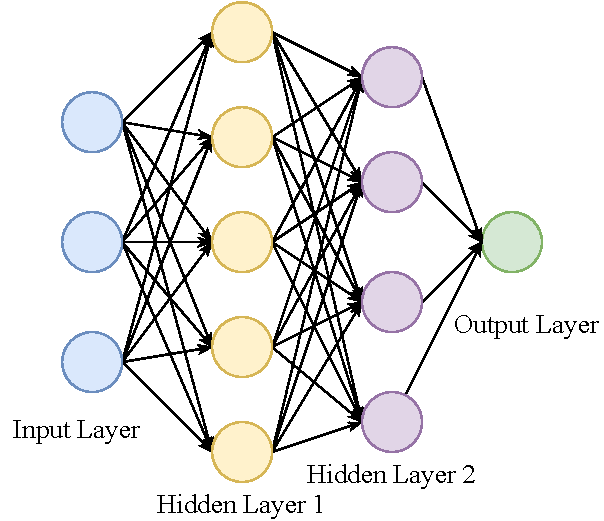
\includegraphics[width=0.4\textwidth]{./figs/fc.pdf}
\caption{An Fully Connected ANN with 2 hidden layers}
\label{fcnn}
\end{figure}
\par
Furthermore, an ANN will be called a Deep Neural Network (DNN) if it has many layers. In more detail, various architectures are introduced for DNN solving different complex problems. Some notable examples are Convolutional Neural Networks (CNNs) and Recurrent Neural Networks (RNNs). The former one is vastly used for video analysis and image classification. Yet, Natural Language Processing is one of use cases for the latter one. 
\par
As has been mentioned before, \smartnics have limited resources. On the other hand, ANNs are resource-hungry applications. Consequently, the original ANNs applications cannot execute on the \smartnics without any modifications. Here, three solutions are listed for reducing the size of any ANNs, including fully connected NNs and DNNs.
\begin{itemize}
  \item \textbf{Compressing}: In this method, the original model is converted to a compressed one via the framework's tools. The compressed one has 2x-4x less size without a prominent loss in the outputs (less than 0.5\% in our results). An example of this method is TensorFlow lite \cite{tflite}.
  \item  \textbf{Quantization}: In this method, more miniature data types are replaced with original data types. In other words, the quantized network has the same topology while the weights of vertices change. In the AI area, using 64bits or 32bits floating-point numbers is very common.  Hence, replacing them with 8bit width data types drops the size significantly. Some studies go further and use only one bit for quantization, generating Binarized Neural Networks (BNNs). It goes without saying that the quantized model is not as accurate as of the original model.
  \item  \textbf{Pruning}: The idea behind this method is to remove the vertices with small weights, or the vertices do not affect the output that much. Therefore, the topology becomes simpler here.
\end{itemize}

Up to here, we have provided adequate background regarding ANNs. The question coming to mind is \textbf{which ANN do we study in our project?}
As we have mentioned, each ANN is suitable for a specific problem. The same in the Computer Networks area; based on the nature of the issue, the ANN's architecture would be chosen. For packet classification, fully connected ANNs provide acceptable accuracy. However, for analysis MPLS configuration, a deep NN provides a viable outcome \cite{8999396}. Here, we will evaluate two kinds. The first one would be VGG16 \cite{simonyan2014very}, which is basically a deep NN for Image Classification. The second one would be a fully connected ANN for anomaly detection. We try to avoid quantizing or pruning the models, and utilizing the original model or the compressed one to keep the models accurate in our project.

\section{Offloading Neural Networks into \textit{SmartNICs}}
\label{sec-motive}

\textcolor{red}{[Talk about the necessities for accelerating NN/DNNs. Introduce the different opportunities/options of accelerators we have (GPU,TPU). Make the case for using SmartNICs as accelerators. Describe the efforts people already did in that sense (this related work, e.g., gianni's paper goes here. Other (less) related work goes into related work section. Mention we want to shed light into the capabilities of SmartNICs as NN accelerators. Give a very high overview of our evaluation and evaluation goals (say we tested different neural network types on different SmartNICs to understand their performance). Evaluation details (i.e., methodology) will be described in the next section).]}

Emerging applications, e.g., Deep Learning based applications - those using DNN and video analytics and image classification, pose a challenge to cloud-based services. These applications demand high network bandwidth and low latency that may not be possible due to the long communication distance between mobile devices and cloud servers. One alternative is to deploy servers closer to mobile users, which is called edge computing. \smartnics also can be used as edge servers providing fast services to the mentioned applications. In a typical fashion without any \smartnic, the NIC, host's CPUs, and GPU/TPU (two standard accelerators for ANN) communicate through PCIe express slot. Once a packet reaches the NIC, it goes through PCIe to CPUs. Then it should be passed to GPU/TPU, again through PCIe. The response should traverse the reverse path, meaning PCIe is passed four times in this scenario. 
\par
What will happen if we execute the model on a \smartnic and avoiding the PCIe slot's overhead. Siracusano \etal \cite{siracusano2020running} conducted novel research focusing on running deep learning applications on \smartnics. The offloading inference phase of three network-based machine learning applications to \smartnics is studied in the mentioned work. They compared three implementations, on Netronome, on P4-NetFPGA, and HDL. In terms of IPC, CPUs of \smartnics are more efficient than hosts'. Therefore, \smartnics are viable candidates for processing those requests. Due to limited resources available in their hardware, they applied Binarized Neural Network to decrease the memory demand and resolving the lack of floating-point operations on \smartnics. However, they lost some accuracy because of quantization. Though, they can offer much higher throughput and less latency by applying their approach.
\par
In the following section, we evaluate different ANNs on a different \smartnic having enough resources and supporting floating-point operations to understand whether we can have quicker latency without losing latency. Moreover, we alleviate the host's CPUs by executing models into the \smartnic.

\section{Measurement setup}
\label{sec-testbed}


\textcolor{red}{[Describe the devices we are evaluating]}

In this section, we addressed our testbed in detail. Firstly, we explain our hardware setup, devices' specs, and how they are connected. Knowing hardware testbed, we explain our software environments. Fig \ref{testbed} shows an overview of both hardware and software of our experiments. Eventually, we speak about our performance metrics.

 \subsection{Hardware Testbed}
As Fig. \ref{testbed} exposes, on the left side, we use an off-path \smartnic equipped with a Cortex-72 ARM CPU working at 800 MHz, with 16 cores and 16GB onboard DDR4 memory. It holds a dual-port SFP28 with 25Gbps for each one. It is mounted on the host, which owns an Intel(R) Xeon(R) Silver 4210R CPU working at 2.4GHz, with 10 cores and 32GB memory. Further details regarding cache are reported in Table \ref{cache-size}. Either the host or the \smartnic act as the server machine connecting to a client over a Tofino switch. The client is equipped with an Intel(R) Core(TM) i7-9700 CPU working at 3.0GHz, with 8 cores and 12GB memory. 
\begin{table}[!htb]
\caption{Size of Cache in the host and \smartnic}
\label{cache-size}
\begin{tabular}{|c|c|c|c|c|}
\hline
Device                         & D-Cache & I-Cache & L2   & L3   \\ \hline
\smartnic (ARM) & 512KB   & 768KB   & 8MB  & 12MB \\ \hline
Host (x86)                     & 320KB   & 320KB   & 10MB & 14MB \\ \hline
\end{tabular}
\end{table}


\subsection{Software Setup}
On the server-side, Ubuntu 20.04.1 LTS with kernel 5.4.0-66-generic is installed on the host. The same OS runs on the client machine, as well. Nonetheless, the \smartnic executes Ubuntu 20.0.1 with a modified kernel 5.4.44. 
\par
For implementing our ANNs, we used two frameworks; 
\begin{itemize}
 \item \textbf{TensorFlow}  \cite{abadi2016tensorflow}: We implemented VGG16 \cite{simonyan2014very} with TensorFlow. Our model recognizes type of pets based on the images. We adopted "Cats vs Dogs" dataset \cite{petimages} to train and test our model. Moreover, we compressed the trained model with TensorFlow lite \cite{petimages}, and ran that version on our \smartnic. Note to mention, both machines support floating-point operation, and we do not apply any quantization method.
 \item \textbf{scikit-learn}  \cite{scikit-learn}: By this framework, we implemented the second used case in \cite{siracusano2020running}, with the same dataset, but without any quantization. The neural network is an MLP classifier for anomaly detection in the UNSW-NB15 dataset \cite{UNSW}, having three layers with the size of (32, 16, 2).
\end{itemize}

\begin{figure}[ht!]
\centering
    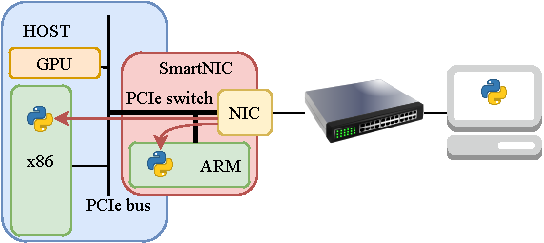
\includegraphics[width=0.47\textwidth]{./figs/testbed.pdf}
    \caption{The testbed}
    \label{testbed}
\end{figure}

\subsection{Workload}
\textcolor{red}{[Describe how we generate the workload in our experiments]}

For evaluating the system, we have developed a socket-based client-server application in Python3. The client program, running on the right-hand machine of Fig. \ref{testbed}, data is read from the dataset; Then, a request is transmitted to the server program, running either on the host or on the \smartnic on the left side Fig. \ref{testbed}, over a TCP connection. The server code runs the model and waits for requests. Once it receives any, it captures and decodes the data, performs the corresponding operations, and finally returns the response to the client. Besides, we can break down the overall latency by adding timestamps in our code. Our implemented codes are released in our Git repository \cite{sdn2021git}

\subsection{Measured resources}
\textcolor{red}{[Describe our metrics and how we measure them in each device]}

Once a neural network is implemented, the first point coming to mind is how accurate it is. With this in mind, in our experiments, we divide our datasets into two parts, training data (80\% of whole data) and test data (the rest 20\% of data). The trained models are evaluated by unseen test data at the end of the training, and the accuracy is measured.
\par
The following parameter reserving some words here is the latency. As we addressed in previous lines, we implemented our code in Python3. We can measure the overall latency in our client program. Once the code sends a request, it also starts the timer. Whenever it captures the response, stops the timer, and calculates the overall latency. With the same timestamping approach, we can break down the latency in the server code to extract communicating time and executing time, as a further illustration. 
\par
To clarify the results, we report roofline results. Roofline, proposed in \cite{10.1007/978-3-319-17248-4_7}, is a benchmark estimating the performance in different levels of caches, memory, and CPU. It reports the maximum bandwidth of caches and memory in terms of GB/s, the maximum computation power of the CPU in terms of GFLPs/sec.


\section{Results}
\label{sec-results}

In this section, we report the results gained in the given testbed. First, we lecture about VGG16's results. Then, we report roofline results to clarify the results we provided. At the end of this section, we express the MLP classifier's results.

\subsection{VGG16's Results}
Our evaluation after training depicts the original model and the lite version have 90.6\% and 90.1\% accuracy, respectively. Besides, Table \ref{vgg16} shows the latencies for VGG16 applications. First, we measured the overall latencies for both the \smartnic and the host. The host is 5x faster to calculate the response with the VGG16 model due to results compared to the \smartnic. Considering this, we break down the overall latency to find out which time slot needs more time.  As we can understand from the fourth column of Table \ref{vgg16}, performing the model operations takes 5x times inside \smartnic's CPU. For better understanding, we perform Roofline benchmark to figure out if the results make sense. The results are reported in Table \ref{roofline-results}. The results in the given table show that the host is 8x-10x quicker than the \smartnic. Since VGG16 is a very deep neural network demanding many complex operations, and the \smartnic has limited resources, the overall latency and computation time for the \smartnic are reasonable.

\begin{table*}[hbt!]
\caption{VGG16's Results}
\label{vgg16}
\begin{tabular}{|c|c|c|c|c|c|}
\hline
Device                         & Framework       & Total Latency & Computation Time & Loading the Image & Communication Time \\ \hline
\smartnic (ARM) & TensorFlow lite & 493.58 ms     & 470.99 ms        & 16.88 ms          & 5.71 ms            \\ \hline
Host (x86)                     & TensorFlow      & 107.05 ms     & 97.98 ms         & 5.21 ms           & 3.86 ms            \\ \hline
\end{tabular}
\end{table*}


\begin{table*}[hbt!]
\caption{Roofline's Results}
\label{roofline-results}
\begin{tabular}{|c|c|c|c|c|c|}
\hline
Device                                   & CPU Bound    & Max L1 Speed & Max L2 Speed & Max L3 Speed & Max DRAM Speed \\ \hline
\smartnic (Arm), One Core & 1.1 GFLOP/s  & 14.5 GB/s    & 4.7 GB/s     & 3.2 GB/s     & 2.4 GB/s       \\ \hline
\smartnic (ARM), 16 Cores & 17.6 GFLOP/s & 231 GB/s     & 19.9 GB/s    & 14.1 GB/s    & 10.6 GB/s      \\ \hline
Host (x86), One Core                    & 9.1 GFLOP/s  & 101.0 GB/s   & 73.2 GB/s    & 36.3 GB/s    & 19.7 GB/s      \\ \hline
Host (x86), 16 Cores                     & 91 GFLOP/s   & 1009.4 GB/s  & 49.9 GB/s    & 35.2 GB/s    & 26.8 GB/s      \\ \hline
\end{tabular}
\end{table*}


\subsection{MLP Classifier's Results}
In these experiments, we load exactly the same model either on the \smartnic or on the host for anomaly detection. Consequently, in both cases, the accuracy is the same, nearby 96.03\%. Since the load for this experiment is not much, we run the server code on one core. In addition to that, we increased the number of connections on the client-side. The measured results are expressed in Table \ref{mlp-results} illustrating how long it takes for the server to respond. Excluding eight connections, both the \smartnic and the host have more or less the same latencies. Averages are less for the \smartnic than the host, while the standard deviation is higher than the host. Once we set the number of connections to eight, the \smartnic works fine, with reasonable changes in the results. However, the host's CPU utilization reaches 100\%; consequently, the connections are refused, and the numbers would not be acceptable anymore.
\par
Further, the communication times demonstrate that the \smartnic would be a good fit for the applications demanding high communication, such as I/O intensive loads. In other words, the \smartnic has faster access to the PCI Express slot than the host; keeping in mind that several devices can be mounted on the host through the slot, and x86 should handle the challenge as well.
\par
Evaluating these applications is beyond our project. Eventually, owing to these results, we can understand, MLP classifiers are a good fit for executing on the \smartnic; one wimpy core of the \smartnic can have the same performance compared to one powerful core of the host.

\begin{table*}[hbt!]
\caption{Average Latencies for the MLP classifier to Detect the Anomaly.}
\label{mlp-results}
\begin{tabular}{|c|c|c|c|c|}
\hline
\multicolumn{5}{|c|}{Average (Standard Deviation) of the Latancies in ms}                   \\ \hline
Device:       & \multicolumn{2}{c|}{\smartnic (ARM)} & \multicolumn{2}{c|}{Host (x86)}      \\ \hline
The Number of Connections & Overall Latency & Communication Time & Overall Latency & Communication Time \\ \hline
1             & 3.89 (2.99)     & 1.14 (0.18)        & 4.01 (1.01)     & 1.67 (0.19)        \\ \hline
2             & 4.00 (7.98)     & 0.62 (0.42)        & 4.02 (1.46)     & 1.69 (0.9)         \\ \hline
4             & 4.2 (19.41)     & 0.2 (0.12)         & 4.6 (3.13)      & 1.10 (1.49)        \\ \hline
8             & 12.56 (31.04)   & 0.47 (4.44)        & N/A             & N/A                \\ \hline
\end{tabular}
\end{table*}

\section{Related work}
\label{sec-related}

\textcolor{red}{Offloading other applications to SmartNICs.}

Many researchers studied different aspects of \smartnics, and how \smartnics can be used wisely to provide better performance even with comparison hosts with powerful CPUs. Long story short, we picked a few of them here.
\par
Ming \etal in \cite{10.1145/3341302.3342079} extended three well-known distributed applications to use the proposed framework's APIs (called iPipe) and benefit \smartnics interests, such as saving up the Host's CPU and more agile latency. The applications explored are a replicated key-value store, a distributed transaction system, and a real-time analytics engine. Furthermore, two on-path and two off-path \smartnics using embedded CPU have been investigated. Characterizing the performance of each \smartnics, they acquainted iPipe framework for distributed applications. The framework providing actor-based programming consists of three major components, an actor scheduler, a distributed memory object abstraction for actor migration, and, eventually, a security isolation mechanism. Carried out experiments manifest that on-path \smartnics show better performance than off-path ones.
\par
Daniel \etal \cite{211249} conferred a solution to offload networking in a virtualized environment into \smartnics and accepted the FPGA-based one as the best decision for both speed and programmability. Single Root I/O Virtualization is introduced in a nutshell, allowing VMs to have direct access to \smartnics. Moreover, the NIC is responsible for all network management. Their given method provided the quickest latency for a public cloud at the time the article was published. 
\par
E3 paper \cite{234944} employed Cavium LiquidIO \smartnics, which is equipped with MIPS architecture CPUs, to offload a few microservice-based applications. The goal, as same as other works, is to reduce the latency and power consumption. In a nutshell, the tool, by knowing the system's topology and eliminating extra overhead, distributes the load among the resources in heterogeneous systems with various architectures, x86, and ARM. The idea is to run microservices on \smartnics as long as enough traffic is passed to the hosts.
\par
Many IoT wireless devices have ultra-limited resources; nevertheless, many deep learning applications hoping to be run on the edge need huge resources; take wireless cameras as an example that captures photos to be processed. Moreover, the network's bandwidth may fluctuate for the devices. CLIO paper \cite{10.1145/3372224.3419215} introduces a prototype for those kinds of tools. Previous papers had tried to either reduce the raw data or compress the models; the accuracy dropped, consequently. Considering a deep learning model, CLIO splits the model, and a part of the model with a few layers is offloaded into devices. Further, different slices, with different sizes, from the last layer have been created. The prototype decides to transmit the best choice based on the available bandwidth. Hence the bandwidth is used efficiently; simultaneously, reasonable accuracy is achieved. Keep in mind that the outputs of middle layers have much less data compared to raw data. 


\section{Conclusion}
\label{sec-conlcu}

In this project, we first talked about \smartnics and a few architectures for them; then, we discussed each architecture has its advantages. However, all of them release resources from the host. So, data center administrators take this advantage to move applications into \smartnic, freeing more resources on the servers for tenants. 
\par
Later, we spoke about the importance of neural networks and their popularity in different applications. Focusing on \smartnic, we provided a project explaining some case studies requiring fast latency and lower bandwidth. In the project, the researchers adopted on-path \smartnics having very limited resources. So, they quantized their neural networks to reduce the model size. However, those \smartnics had not supported floating-point operations. Their limitations lead them to use binarized neural networks,  losing accuracy and being compatible with the devices.
\par
In this project, we chose an off-path \smartnic which has more resources and supports floating-point operations. Therefore we do not lose accuracy more than 0.05\%. Our results show that ARM-based \smartnics still have limited resources and computation power than the hosts, and they are not a suitable environment for executing complex neural networks such as VGG16. Running VGG16 on our \smartnic takes approximately 5x more time than the host. Conversely, ARM-based \smartnics would be competitive resources for executing simpler neural networks such as MLP classifiers due to their quicker communication time. We were able to offload a workload running on one core of the host to one core of the \smartnic, without any change in the outputs, and still have more space in the \smartnic.

\bibliographystyle{ACM-Reference-Format}
\bibliography{reference}

\end{document}